\documentclass{article}\usepackage[]{graphicx}\usepackage[]{color}
%% maxwidth is the original width if it is less than linewidth
%% otherwise use linewidth (to make sure the graphics do not exceed the margin)
\makeatletter
\def\maxwidth{ %
  \ifdim\Gin@nat@width>\linewidth
    \linewidth
  \else
    \Gin@nat@width
  \fi
}
\makeatother

\definecolor{fgcolor}{rgb}{0.345, 0.345, 0.345}
\newcommand{\hlnum}[1]{\textcolor[rgb]{0.686,0.059,0.569}{#1}}%
\newcommand{\hlstr}[1]{\textcolor[rgb]{0.192,0.494,0.8}{#1}}%
\newcommand{\hlcom}[1]{\textcolor[rgb]{0.678,0.584,0.686}{\textit{#1}}}%
\newcommand{\hlopt}[1]{\textcolor[rgb]{0,0,0}{#1}}%
\newcommand{\hlstd}[1]{\textcolor[rgb]{0.345,0.345,0.345}{#1}}%
\newcommand{\hlkwa}[1]{\textcolor[rgb]{0.161,0.373,0.58}{\textbf{#1}}}%
\newcommand{\hlkwb}[1]{\textcolor[rgb]{0.69,0.353,0.396}{#1}}%
\newcommand{\hlkwc}[1]{\textcolor[rgb]{0.333,0.667,0.333}{#1}}%
\newcommand{\hlkwd}[1]{\textcolor[rgb]{0.737,0.353,0.396}{\textbf{#1}}}%
\let\hlipl\hlkwb

\usepackage{framed}
\makeatletter
\newenvironment{kframe}{%
 \def\at@end@of@kframe{}%
 \ifinner\ifhmode%
  \def\at@end@of@kframe{\end{minipage}}%
  \begin{minipage}{\columnwidth}%
 \fi\fi%
 \def\FrameCommand##1{\hskip\@totalleftmargin \hskip-\fboxsep
 \colorbox{shadecolor}{##1}\hskip-\fboxsep
     % There is no \\@totalrightmargin, so:
     \hskip-\linewidth \hskip-\@totalleftmargin \hskip\columnwidth}%
 \MakeFramed {\advance\hsize-\width
   \@totalleftmargin\z@ \linewidth\hsize
   \@setminipage}}%
 {\par\unskip\endMakeFramed%
 \at@end@of@kframe}
\makeatother

\definecolor{shadecolor}{rgb}{.97, .97, .97}
\definecolor{messagecolor}{rgb}{0, 0, 0}
\definecolor{warningcolor}{rgb}{1, 0, 1}
\definecolor{errorcolor}{rgb}{1, 0, 0}
\newenvironment{knitrout}{}{} % an empty environment to be redefined in TeX

\usepackage{alltt}
\usepackage[margin =1in]{geometry}
\usepackage{placeins}
\title{Additional Simulations for High Dimensional LiNGAM}
\author{}
\IfFileExists{upquote.sty}{\usepackage{upquote}}{}
\begin{document}
\maketitle

\section{Procedure}
Specifically, for the pairwise LiNGAM + preselection procedure we do-

\begin{enumerate}
\item Use cv-lasso to select the neighborhood for each node. We make the skeleton by using "or-rule."
\item Then following following Hyvarinen and Smith (2013), we use the pairwise statistic (without any additional conditioning) to assign a direction for each edge in the estimated skeleton.
\item  We estimate each edge weight using OLS
\item As suggested by Hyvarinen and Smith (2013), we use the ordering procedure from Alg B and Alg C of Shimizu et. al (2006) which uses a progressively larger threshold for the edgeweights until a total ordering can be achieved. If there are multiple possible roots, the existing code (by Jonas in the pcalg package) simply takes the first one (i.e., matches the ordering from the input matrix). So if we set all edgeweights to 0, with the existing code we would still get kendall's tau of 1. So I changed the code slightly to select a root at random if multiple roots are possible since in our setup there is always a single root that we would choose.
\end{enumerate}

For our procedure + preselection, we also do step (1). We then run the normal procedure but limit the set of possible parents for each node to the estimated neighborhood. 

\FloatBarrier

\section{Results}

In the graph, the x-axis shows p, the number of nodes and $n$ the number of samples is always 3/4p. The dark boxplots are HDL (our high dimensional lingam procedure without any pre-selection), the light-gray boxplots are HDL+p (our high dimensional lingam + pre-selection), and the white boxplots are PW+P (the pairwise procedure from Hyvarinen and Smith + pre-selection). In general the ordering of performance is HDL+P, HDL, and PW+P. Although, our procedure knows the max-indegree so we'd expect it to do a bit better. From the graphs, it appears that everyone does better in the hub setting, but recall that we had to make the simulation settings slightly easier in the hub case so that consistency can be shown. Thus, the two settings are not directly comparable.


\begin{knitrout}
\definecolor{shadecolor}{rgb}{0.969, 0.969, 0.969}\color{fgcolor}

{\centering 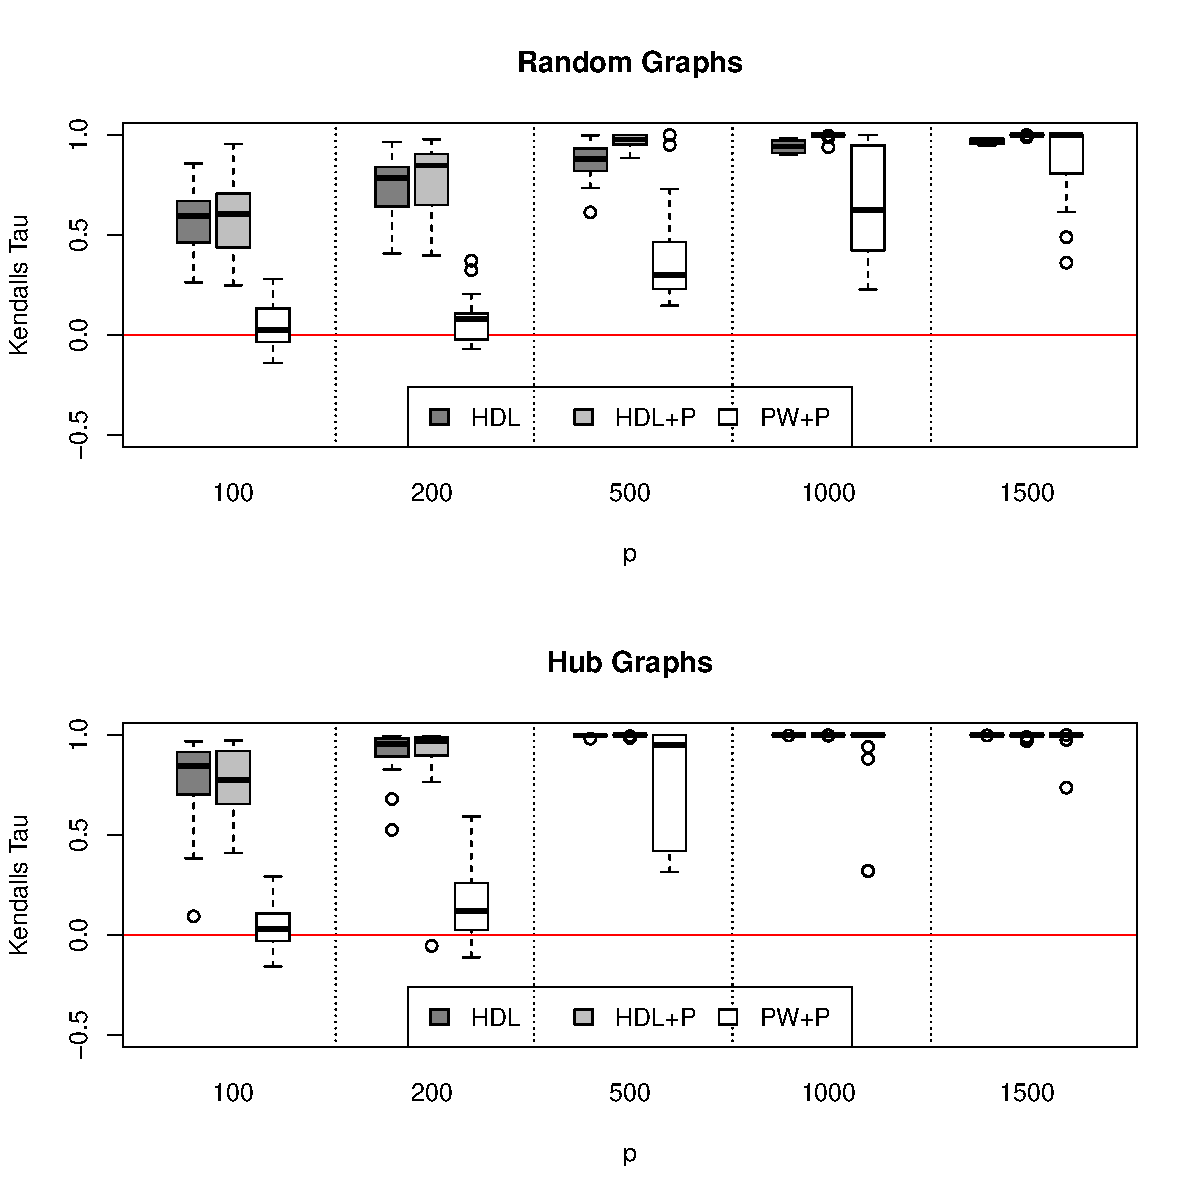
\includegraphics[width=\maxwidth]{figure/unnamed-chunk-1-1} 

}



\end{knitrout}



The performance of PW+P, even though it is last, is still surprisingly good. If we look at the \% of times that the PW+P procedure orients edges in the right direction (i.e., not necessarily a true edge, but at least pointing downstream), we see that it consistently gets roughly 55\% correct and doesn't go above that even as the sample size increases. However, when we use OLS to estimate the magnitude of the edges, the incorrectly oriented edges tend to have a smaller absolute value. Thus, even though we are orienting the edge correclty only 55\% of the time, the incorrect edges get thresholded away when we order the nodes into a DAG and so PW+P still seems to do reasonably well as measured by Kendall's tau. Below is an example of the absolute value of the edgeweights for the correct and incorrect edges. The data is from run one of $p = 1000$ with the hub graph setting. All the edgweights for the incorrect edges are clustered around 0, whereas for the correct edges there is a group around (.5, 1). 

\begin{knitrout}
\definecolor{shadecolor}{rgb}{0.969, 0.969, 0.969}\color{fgcolor}

{\centering 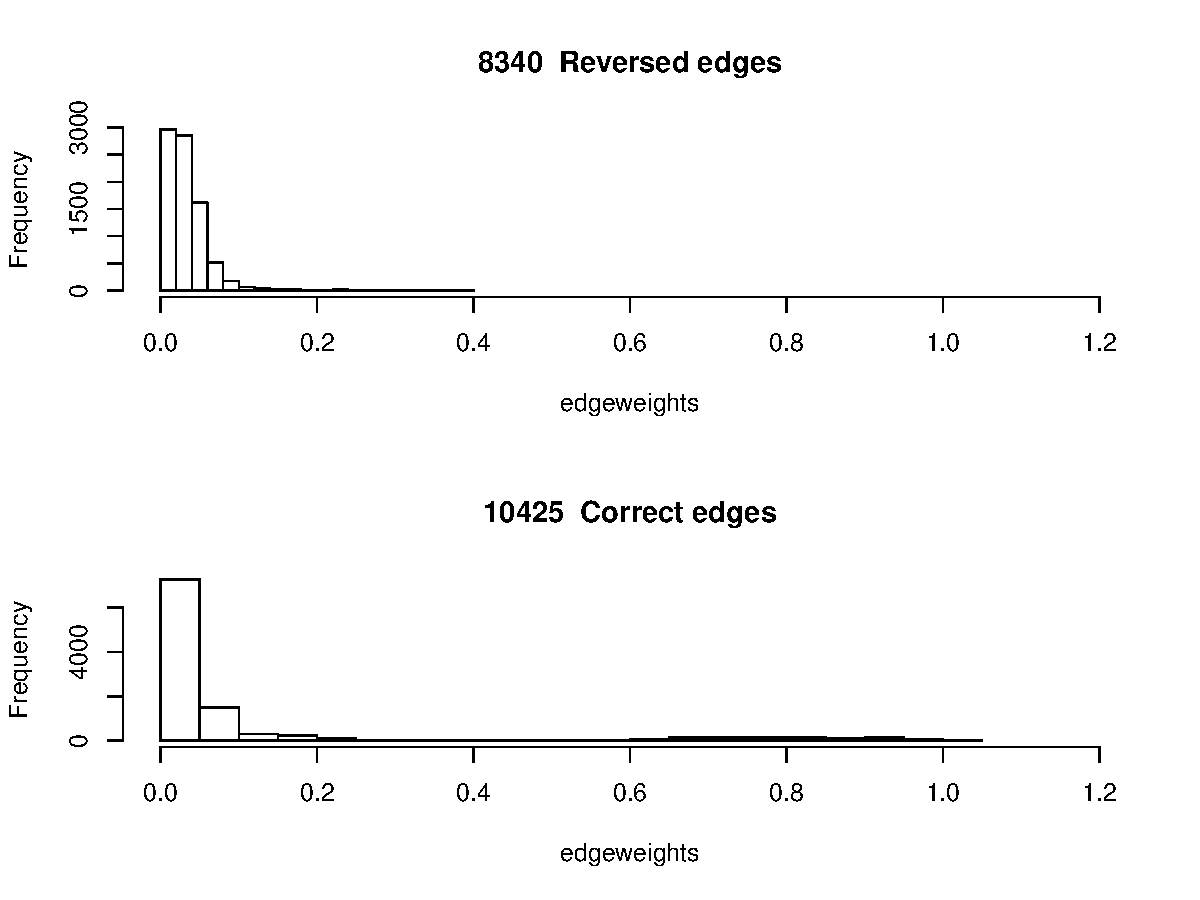
\includegraphics[width=\maxwidth]{figure/unnamed-chunk-2-1} 

}



\end{knitrout}
 

 


\end{document}
